\appendix
\begin{appendices}
    \chapter{Material für Nutzerstudie}
    \label{appendix:study_material}
    Alle hier aufgeführten Materialien sind auch auf der beiliegenden DVD enthalten.
    
    \section*{Flyer für Nutzerstudie}
    \label{appendix:study_flyer}
    \begin{center}
        \framebox[\width]{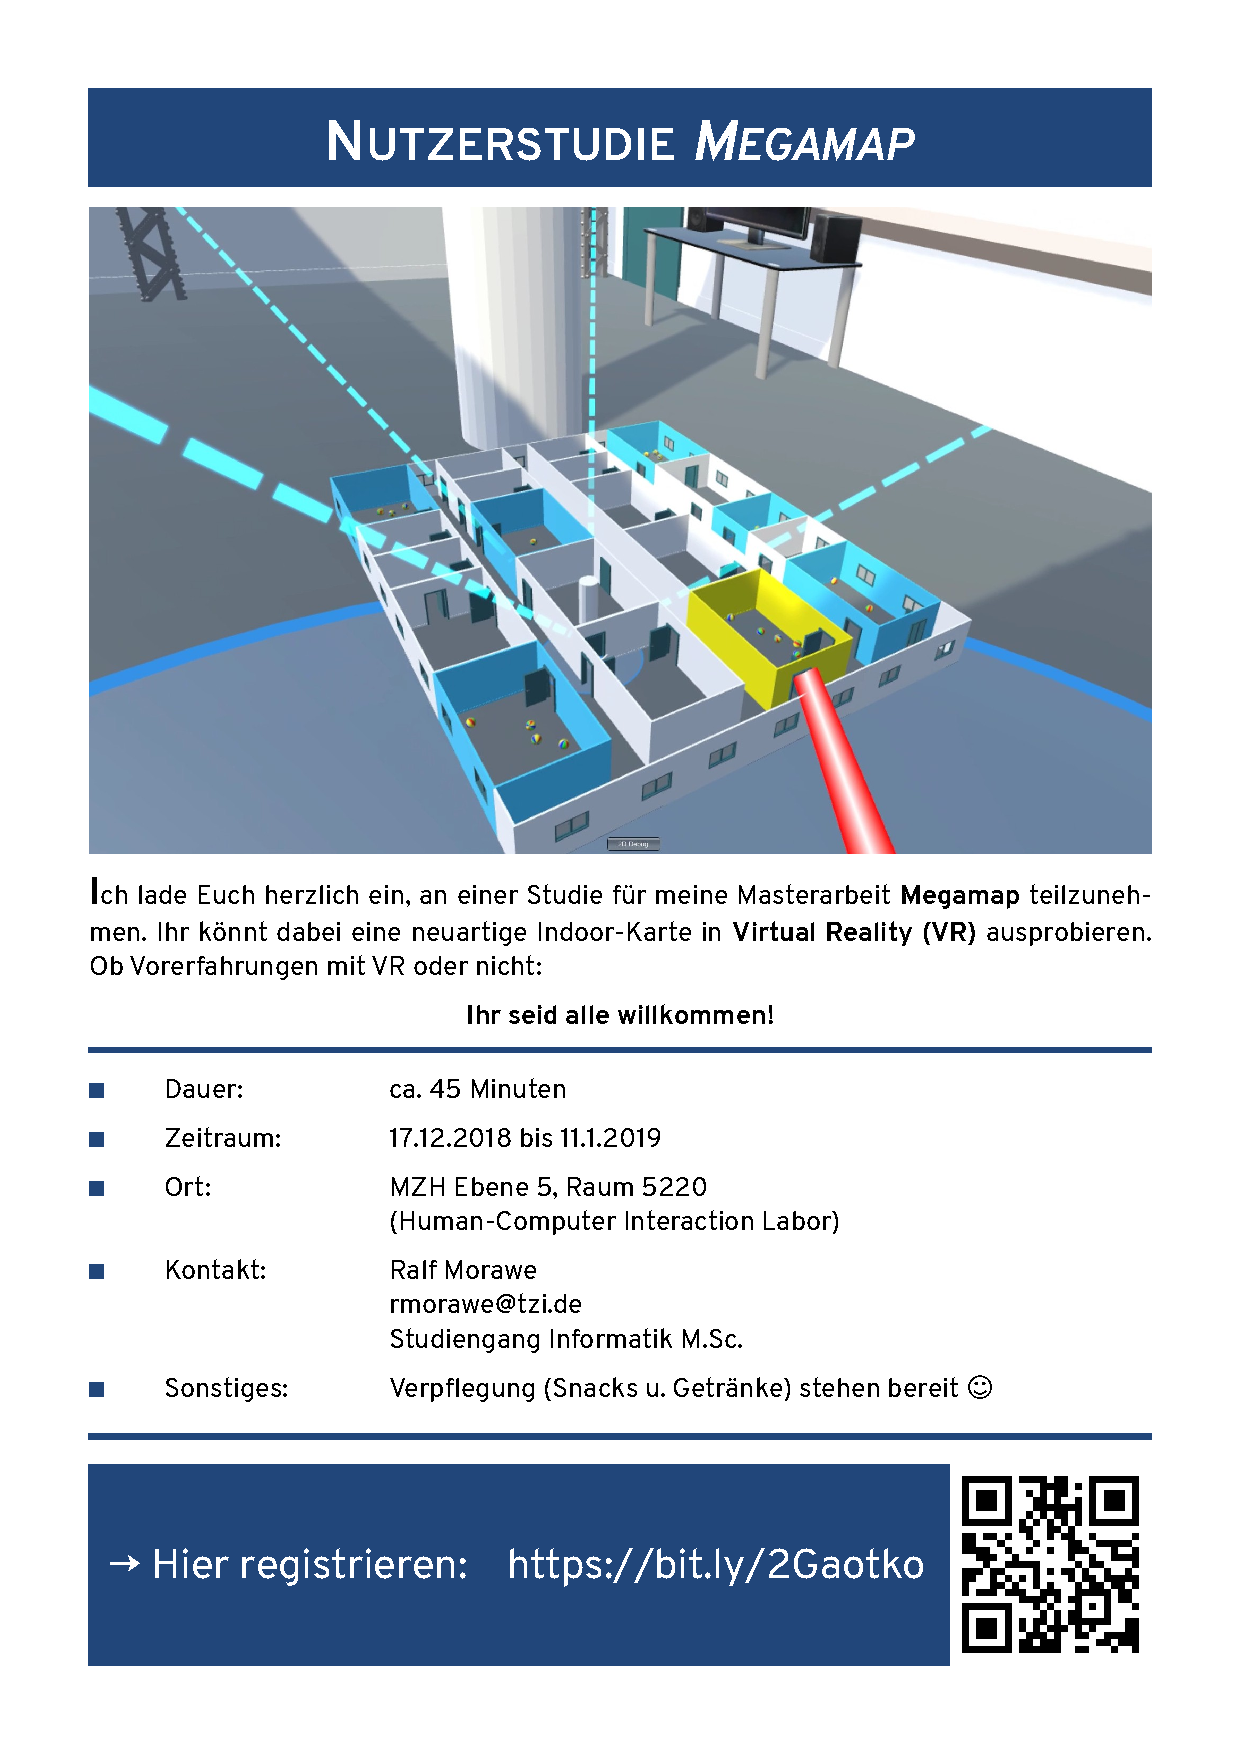
\includegraphics[width=0.6\linewidth]{appendix/study_flyer}}
    \end{center}
    
    \section*{Informationsbogen für Probanden}
    \label{appendix:study_infos}
    \begin{center}
        \framebox[\width]{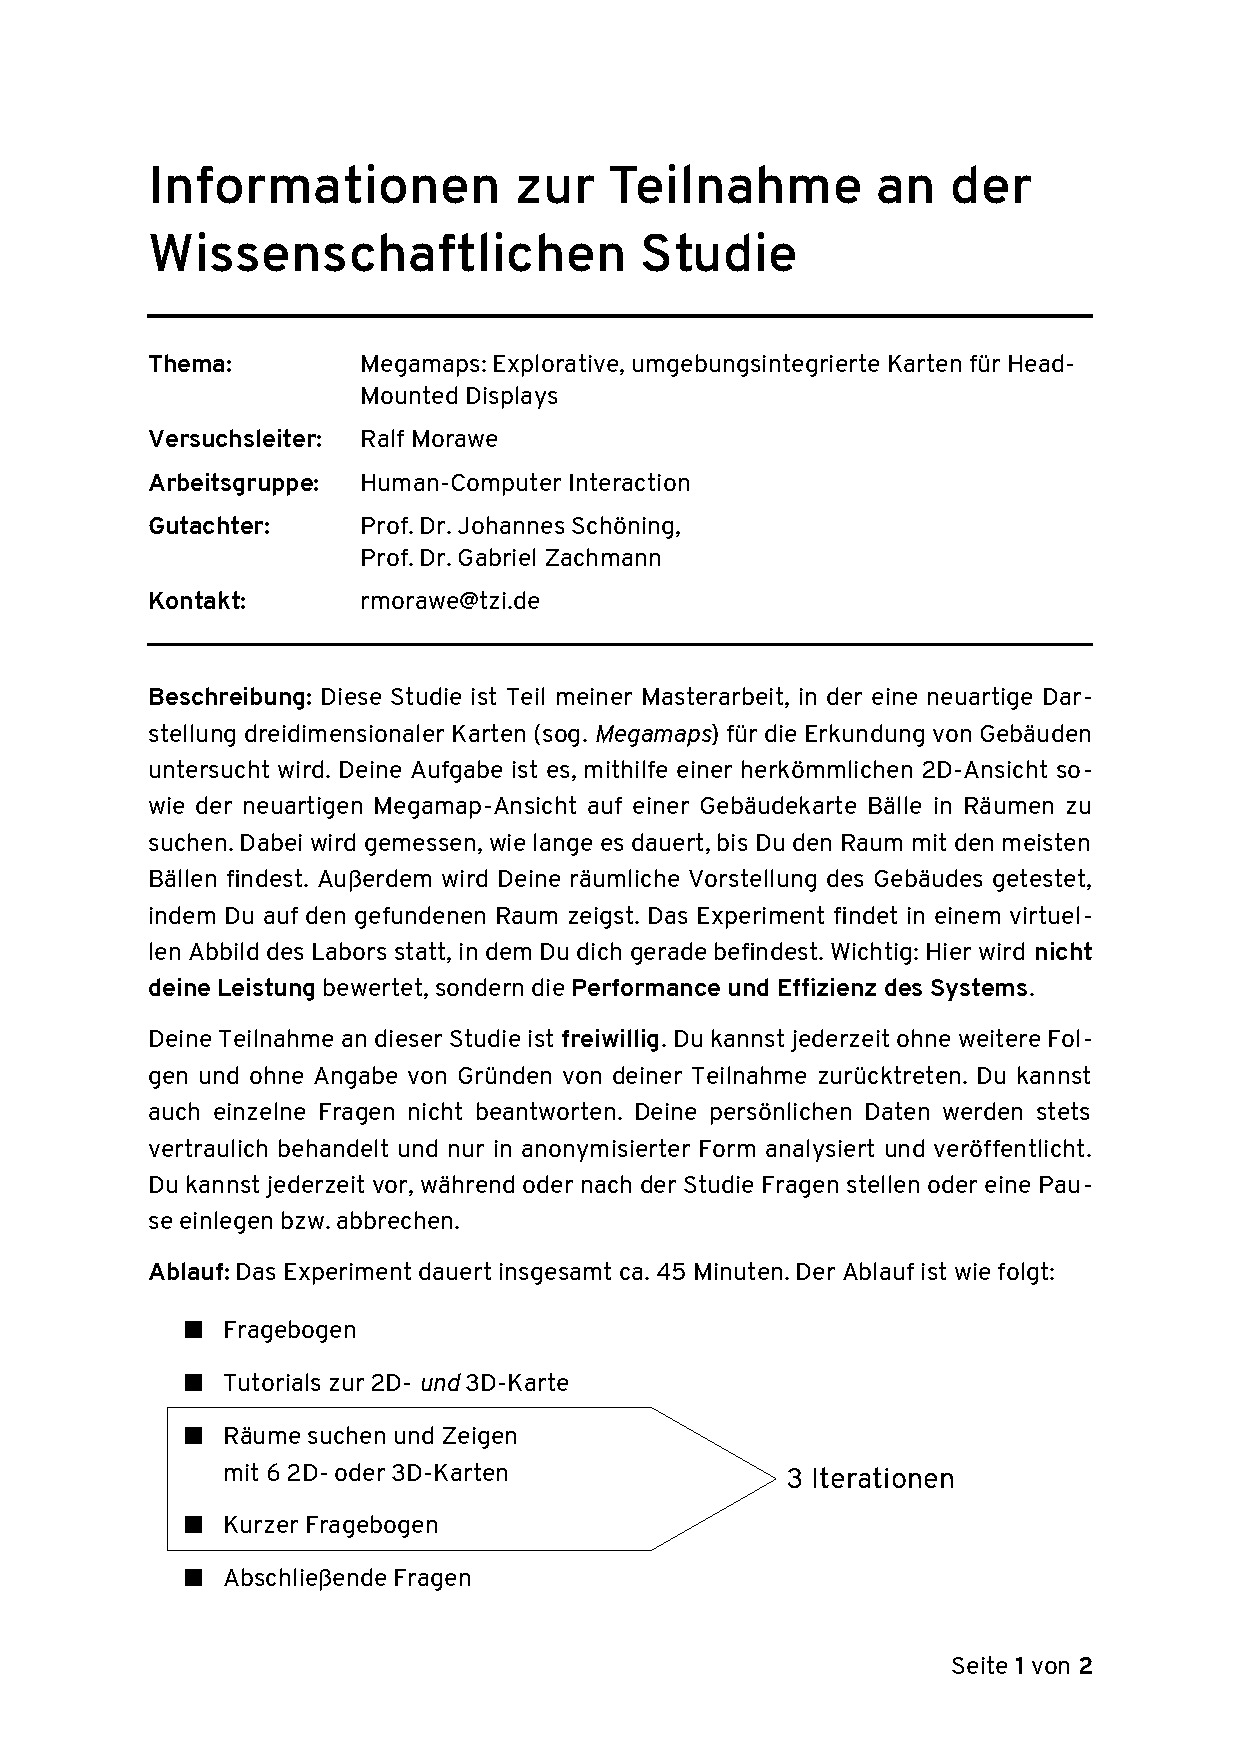
\includegraphics[page=1, trim={2cm, 2cm, 2cm, 2cm}, clip, width=0.58\linewidth]{appendix/study_infos}}
        
        \framebox[\width]{\includegraphics[page=2, trim={2cm, 15cm, 2cm, 2cm}, clip, width=0.58\linewidth]{appendix/study_infos}}
    \end{center}
    
    \section*{Zustimmungsbogen}
    \label{appendix:study_consent}
    \begin{center}
        \framebox[\width]{
\includegraphics[width=0.95\linewidth]{appendix/Zustimmung-Studienteilnahme}}
    \end{center}
    
    \section*{Demografischer Fragebogen und Santa Barbara Sense-of-Direction Skala}
    \label{appendix:demographic}
    Dies ist eine Offline-Variante des eigentlichen Fragebogens, den die Probanden über Google~Forms ausfüllten.
    \begin{center}
        \framebox{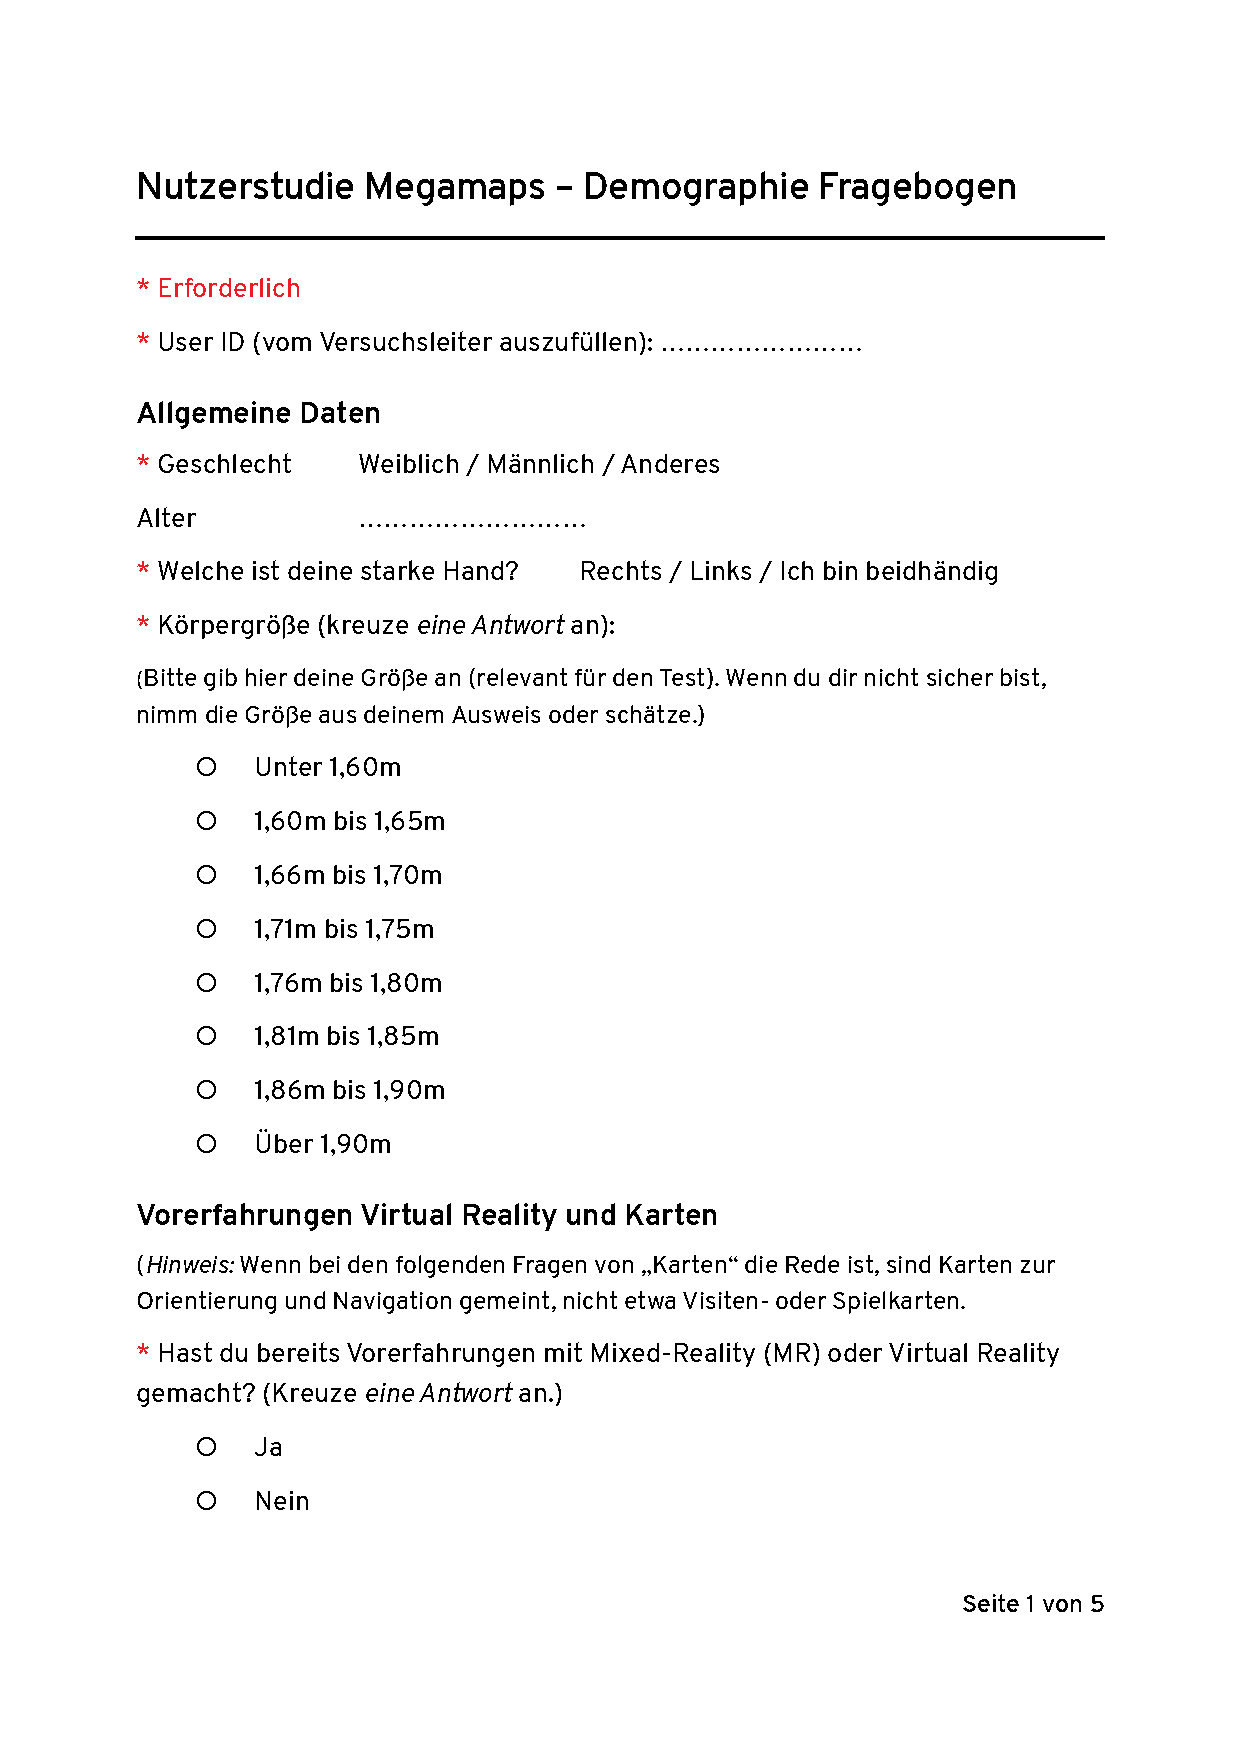
\includegraphics[page=1, trim={1cm, 2cm, 1cm, 2cm}, clip, width=0.8\linewidth]{appendix/demographie_fragebogen}}
    \end{center}
    
    \begin{center}
        \framebox[\linewidth]{\includegraphics[page=2, trim={1cm, 2cm, 1cm, 2cm}, clip, width=\linewidth]{appendix/demographie_fragebogen}}
    \end{center}
    
    \begin{center}
        \framebox[\linewidth]{\includegraphics[page=3, trim={1cm, 2cm, 1cm, 2cm}, clip, width=\linewidth]{appendix/demographie_fragebogen}}
    \end{center}
    
    \begin{center}
        \framebox[\linewidth]{\includegraphics[page=4, trim={1cm, 2cm, 1cm, 2cm}, clip, width=\linewidth]{appendix/demographie_fragebogen}}
    \end{center}
    
    \begin{center}
        \framebox[\linewidth]{\includegraphics[page=5, trim={1cm, 2cm, 1cm, 2cm}, clip, width=\linewidth]{appendix/demographie_fragebogen}}
    \end{center}
    
    \section*{Fragebogen zu den Konditionen $\bm{3D_l}$, $\bm{3D_h}$ und $\bm{2D}$}
    \label{appendix:sus}
    Dies ist eine Offline-Variante der eigentlichen Fragebogen, die die Probanden über Google~Forms ausfüllten.
    
    \begin{center}
        \framebox[\width]{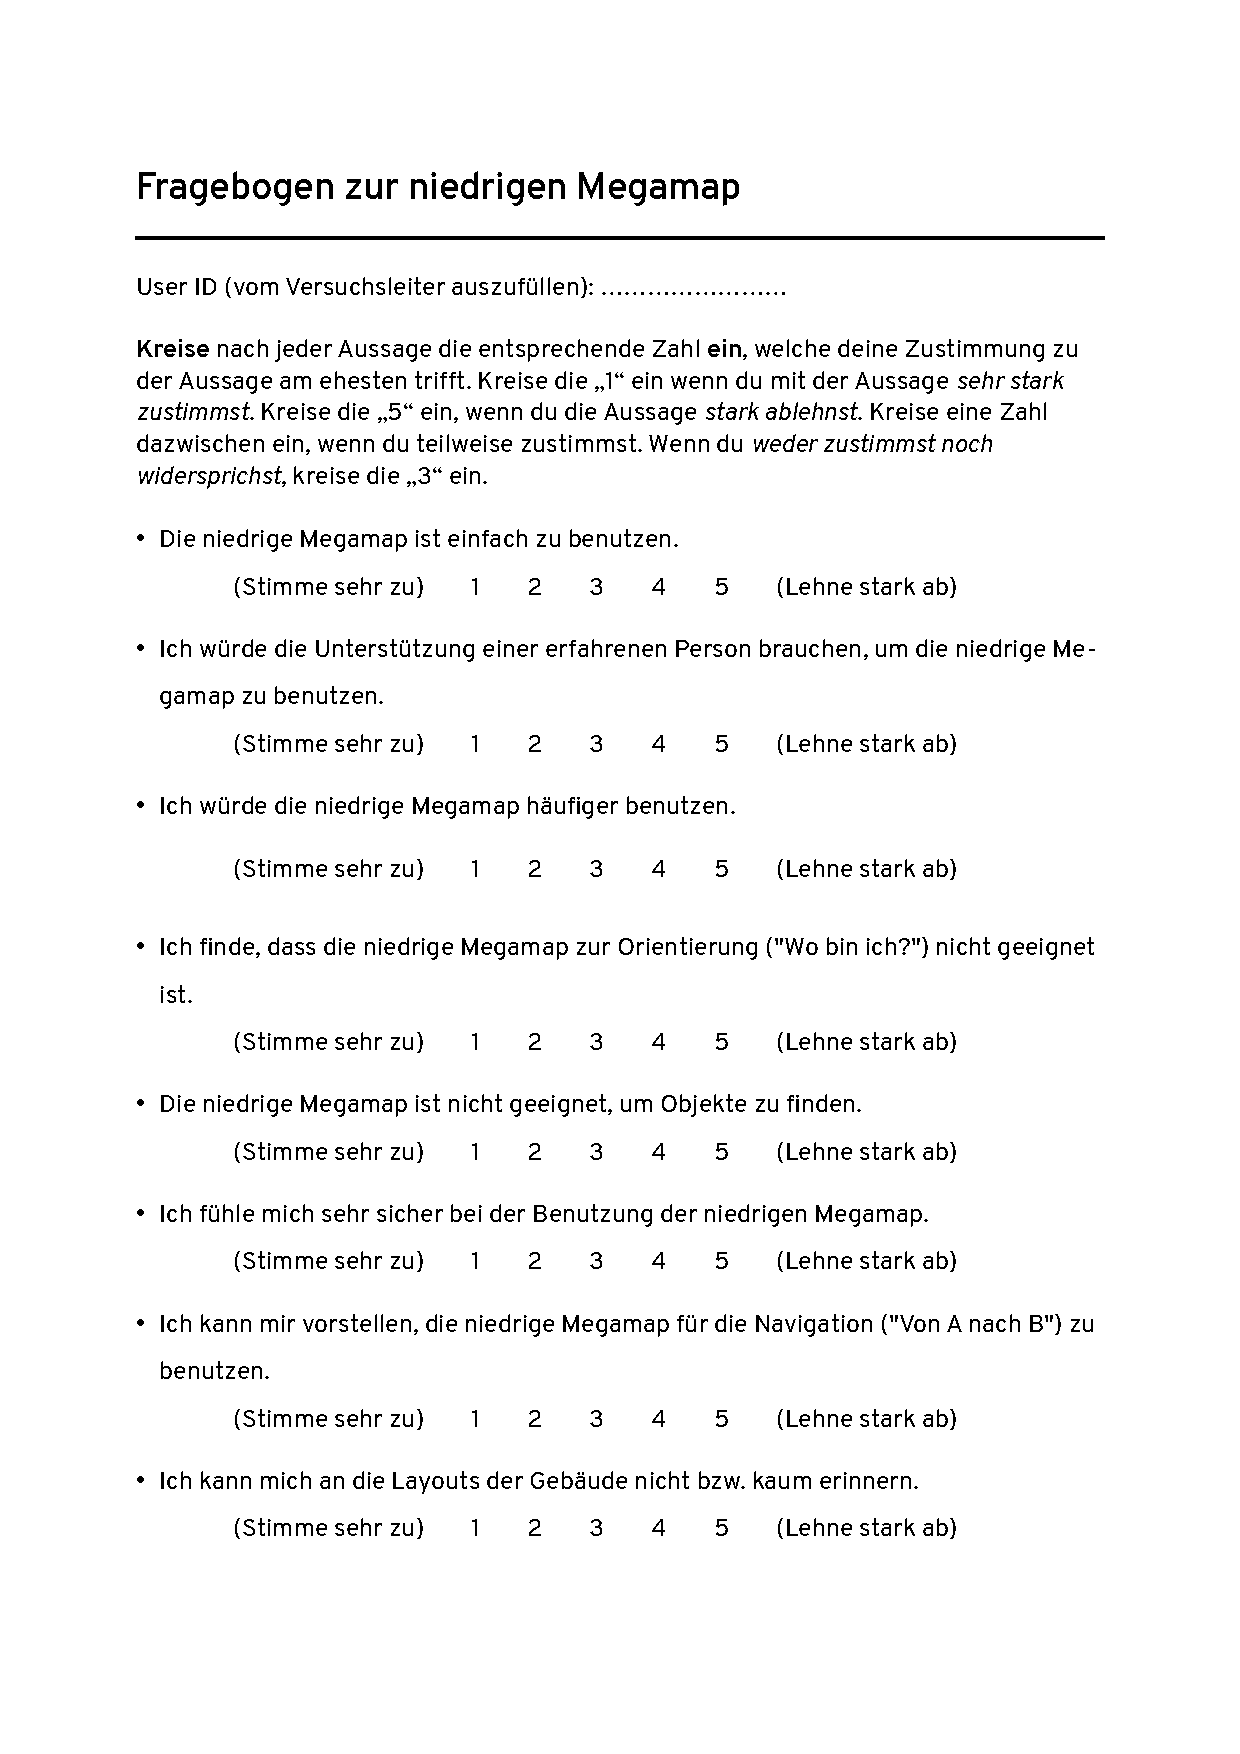
\includegraphics[page=1, trim={1cm, 2cm, 1cm, 2cm}, clip, width=0.85\linewidth]{appendix/fragebogen_megamap}}
    \end{center}
    \clearpage
    
    \begin{center}
        \framebox[\linewidth]{\includegraphics[page=2, trim={1cm, 2cm, 1cm, 2cm}, clip, width=\linewidth]{appendix/fragebogen_megamap}}
    \end{center}
    \clearpage
    
    \begin{center}
        \framebox[\linewidth]{\includegraphics[page=3, trim={1cm, 2cm, 1cm, 2cm}, clip, width=\linewidth]{appendix/fragebogen_megamap}}
    \end{center}
    \clearpage
    
    \section*{Fragen für Leitfadeninterview}
    \label{appendix:interview}
    \vspace{2em}
    \begin{itemize}
        \item Welche Kartenvariante war dein Favorit für \emph{die Suche}?
        
        \item Welche Kartenvariante war dein Favorit für \emph{die Richtungsschätzung}?
        
        \item Hast du die Room-Guides bemerkt bzw. zur Orientierung genutzt?
        
        \item Was war dein Vorgehen bei der Suche?
        
        \item Wie hast du dir die Richtungen zum Zielraum gemerkt?
        An welchen Punkten hast du dich orientiert?
        
        \item Könntest du dir die Megamap in einer MR-Anwendung für die Exploration von Gebäuden (z.\,B. die Uni~Bremen oder ein Einkaufszentrum) vorstellen?
        Würdest du die MR-Megamap benutzen?
        
        \item Könntest du dir die Megamap in einer MR-Anwendung für die Exploration von \emph{Außenbereichen} vorstellen?
        
        \item Was bräuchte die Megamap deiner Meinung nach, um als Karte benutzbar zu sein?
    \end{itemize}
    
    \chapter{Konditionssequenzen für die Nutzerstudie}
    \begin{table}[h!]
        \centering
        \caption{Liste der Konditionssequenzen für die Probanden.}
        \label{appendix:condition_sequences}
        \begin{tabular}{cccc}\toprule
            Proband & Kondition 1 & Kondition 2 & Kondition 3 \\\midrule
            $P_0$ & $3D_l$ & $3D_h$ & $2D$ \\
            $P_1$ & $3D_h$ & $3D_l$ & $2D$ \\
            $P_2$ & $2D$ & $3D_l$ & $3D_h$ \\
            $P_3$ & $3D_l$ & $2D$ & $3D_h$ \\
            $P_4$ & $3D_h$ & $2D$ & $3D_l$ \\
            $P_5$ & $2D$ & $3D_h$ & $3D_l$ \\
            $P_6$ & $3D_h$ & $2D$ & $3D_l$ \\
            $P_7$ & $3D_l$ & $3D_h$ & $2D$ \\
            $P_8$ & $3D_h$ & $3D_l$ & $2D$ \\
            $P_9$ & $2D$ & $3D_l$ & $3D_h$ \\
            $P_{10}$ & $3D_l$ & $2D$ & $3D_h$ \\
            $P_{11}$ & $2D$ & $3D_h$ & $3D_l$ \\
            $P_{12}$ & $3D_l$ & $3D_h$ & $2D$ \\
            $P_{13}$ & $3D_h$ & $2D$ & $3D_l$ \\
            $P_{14}$ & $2D$ & $3D_l$ & $3D_h$ \\\bottomrule        
        \end{tabular}
    \end{table}

    \chapter{Inhalt der DVD}
\end{appendices}